\documentclass[10pt, a4paper]{extarticle}

%%% Работа с русским языком
% правильно: fontspec + polyglossia 
% не надо загружать mathtext, и без него русский в формулах читается,
% зато он конфликтует с polyglossia

% не надо etex
% только newcommand вместо def


%%% Дополнительная работа с математикой
\usepackage{amsfonts,amssymb,amsthm,mathtools} % AMS
\usepackage{amsmath}
\usepackage{icomma} % "Умная" запятая: $0,2$ --- число, $0, 2$ --- перечисление


% https://tex.stackexchange.com/questions/73684
% решаем конфликт amssymb vs dingbat за checkmark
\usepackage{savesym}


\usepackage{caption}
\usepackage{geometry} 
\geometry{left=2cm}
\geometry{right=2cm}
\geometry{top=2cm}
\geometry{bottom=2cm}
% \usepackage[misc,clock, weather, alpine]{ifsym}

\usepackage{graphicx}

%% Шрифты
% \usepackage{euscript}	 % Шрифт Евклид
% \usepackage{mathrsfs} % Красивый матшрифт



%%% Работа с картинками
\setlength\fboxsep{3pt} % Отступ рамки \fbox{} от рисунка
\setlength\fboxrule{1pt} % Толщина линий рамки \fbox{}
\usepackage{wrapfig} % Обтекание рисунков и таблиц текстом

%%% Работа с таблицами
\usepackage{array,tabularx,tabulary,booktabs} % Дополнительная работа с таблицами
\usepackage{longtable}  % Длинные таблицы
\usepackage{multirow} % Слияние строк в таблице
% \usepackage{upgreek}

% \usepackage{enumerate}
\usepackage{dsfont}
\usepackage{todonotes}




%%% Гиперссылки

\usepackage{xcolor}
\usepackage{hyperref}
%\definecolor{linkcolor}{HTML}{8b00ff} % цвет ссылок
\definecolor{linkcolor}{HTML}{120a8f} % цвет ссылок (лучше смотрится с ss)
\definecolor{urlcolor}{HTML}{6b039b} % цвет гиперссылок
\definecolor{citecol}{HTML}{8a2be2} % ссылки на литру

\hypersetup{pdfstartview=FitH,  linkcolor=linkcolor,urlcolor=urlcolor, citecolor=citecol, colorlinks=true}


%%% Заголовок
\usepackage{fancyhdr}
%\setlength{\headheight}{14.2pt}
%\pagestyle{fancyplain}
\pagestyle{fancy}
\fancyhf{}
\fancyhead[L]{\leftmark}
\fancyhead[R]{\thepage}

%\usepackage{minted}

\usepackage{fontspec} 
\usepackage{polyglossia} % для выбора языка в xelatex
\setmainlanguage{russian}
\setotherlanguages{english}

% Ligatures=TeX is on by default
% https://tex.stackexchange.com/questions/323542/
\setmainfont[Ligatures=TeX]{Cantarell}
%\newfontfamily{\cyrillicfonttt}{Times New Roman}
\newfontfamily\cyrillicfont{Cantarell}[Script=Cyrillic]
\setsansfont[Ligatures=TeX]{Cantarell}
\newfontfamily\cyrillicfontsf{Cantarell}[Script=Cyrillic]
\setmonofont{Courier New}
\newfontfamily\cyrillicfonttt{Courier New}[Script=Cyrillic]



\usepackage[sf,sl,outermarks]{titlesec}
\titleformat{\section}
{\LARGE\sffamily}
{\thesection}{0.5em}{}

\usepackage{csquotes}

\usepackage{verbatim}
\usepackage{comment}


%\graphicspath{{images/}{../images/}}
%\usepackage{subfiles}


%\usepackage[bibencoding = auto,
%backend = biber,
%sorting = none,
%style=alphabetic]{biblatex}
\usepackage[backend=biber,bibencoding=utf8,sorting=nty,maxcitenames=4,style=numeric-verb]{biblatex}
\addbibresource{lit.bib}
\usepackage{csquotes}

\title{Сравнение методов визуализации данных}
\author{Карпова Анастасия (БЭК 165) \\ Омелюсик Владимир (БЭК 161)}

\linespread{1.5}

\renewcommand{\le}{\leqslant}
\renewcommand{\ge}{\geqslant}
\renewcommand{\leq}{\leqslant}
\renewcommand{\geq}{\geqslant}

\newcommand{\code}[1]{\texttt{#1}}

\renewcommand{\L}{\mathrm{L}}
\newcommand \mL{\mathcal{L}}
\newcommand{\lsum}{\sum\limits}
\newcommand \R{\mathbb{R}}

\setlength{\parskip}{1em}
\setlength{\parindent}{0cm}

\usepackage{tocloft}
\renewcommand{\cftsecfont}{\hspace{4.5em}\normalfont}
\renewcommand{\cftsubsecfont}{\hspace{5em}\normalfont}
\renewcommand{\cftsecpagefont}{\normalfont\hfill}
\renewcommand{\cfttoctitlefont}{\large\normalfont\hfill}
\renewcommand{\cftaftertoctitle}{\hfill}
\renewcommand{\cftsecleader}{\cftdotfill{\cftdotsep}}


\renewcommand{\cftsecafterpnum}{\hspace*{5.5em}\hfill}
\renewcommand{\cftsubsecafterpnum}{\hspace*{5.5em}\hfill}
\renewcommand{\cftsecaftersnum}{.}
\renewcommand{\cftsubsecaftersnum}{.}


\usepackage{framed}
\definecolor{shadecolor}{gray}{0.9}

\begin{document}

\maketitle
\vspace{-1.1cm}
\tableofcontents
\vspace{1em}
\thispagestyle{empty}

Методы снижения размерности данных разрабатывались с тридацатых годов прошлого века. 
Первые алгоритмы, такие как PCA (Hotelling, 1933) и классический вариант MDS (Torgerson, 1952), были линейными.
В их основу была положена идея, что точки, значительно удалённые друг от друга в исходном пространстве, должны оставаться на большом расстоянии в новом пространстве меньшей размерности \cite{maaten2008visualizing}. 
Таким образом, линейные методы сохраняли глобальные особенности структуры данных. 

Тем не менее, на практике исходное пространство далеко не всегда является линейным, а может представлять собой многообразие сложной формы.
В этой связи часто возникает ситуация, когда важно сохранить, скорее, не глобальные, а локальные свойства данных. 
Например, в биологии молекулы могут кодироваться высокоразмерными векторами, отражающими их свойства, и при снижении размерности важно, чтобы близколежащие молекулы оставались локально различимыми в новом пространстве \cite{tmap}. 
Так как линейные методы не способны справиться с этой задачей, в последние годы активно развиваются нелинейные методы снижения размерности.

Одной из задач, которую можно решить при помощи понижения размерности, является визуализация многомерных данных.
Её суть заключается в  проецировании исходных данных на пространство размерности не выше трёх и последующее изображение векторов в этом пространстве. 
Тем не менее, у задачи визуализации многомерных данных есть некоторые специфические особенности. 
Во-первых, качественная визуализация должна быть понятной и доносить до наблюдателя релевантную (чтобы это не значило) информацию об исходном пространстве.
Во-вторых, не очень понятно, каким образом оценивать и измерять качество визуализации.
Критерии «хорошей картинки» могут варироваться от задачи к задаче.

В этом обзоре будут рассмотрены некоторые методы понижения размерности и их применение для визуализации данных.
Кроме того, будут приведены примеры метрик, используемых для сравнения их качества. 
В связи с популярностью нелинейных методов, большая часть обзора посвящена им. 
Также в работе приведен пример снижения размерности с помощью MDS — одного из наиболее популярных линейных методов после всем известного метода главных компонент (PCA). 

\section{Описание методов визуализации}

\subsection{MDS}

Методы многомерного шкалирования (multidimensional scaling) для снижения размерности данных разрабатывались c пятидесятых годов прошлого века. В этом разделе будет представлен краткий обзор этих методов, а более полную информацию о них можно найти, например, в статье Buja et al. (2008) \cite{buja2008data}.

Основная идея всех методов MDS заключается в том, чтобы отобразить точки из исходного признакового пространства в пространство меньшей размерности таким образом, чтобы попарное расстояние между точками в новом пространстве было как можно более близко к расстоянию между ними в исходном пространстве. Формально, расстояние в исходном пространстве задано «матрицей расхождений» (matrix of dissimilarities) $D = \{d_{i, j} \}_{i, j = 1}^{N}$, а цель алгоритма заключается в поиске векторов $x_1, \ldots x_N \in \R^k$, таких что $d_{i, j}$ хорошо приближается значением $||x_i - x_j||$. Для целей визуализации $k$ выбирается не больше трёх. В классической постановке векторы подбираются таким образом, чтобы минимизировать функцию стресса  (stress function) \cite{kruskal1964multidimensional}.
\[
\text{Stress}_D(x_1, \ldots x_N) = \left( \sum_{i \ne j = 1\ldots N} (d_{i, j} - ||x_i - x_j||)^2  \right)^{1/2}.
\]
Оптимизация происходит применением градиентного спуска в пространстве новых признаков. Матрица $D$ обычно предполагается симметричной. 

Методы MDS различаются, в основном, спецификацией функции потерь. Выделяются два ортогональных вектора различий:
\begin{enumerate}
	\item Классическое шкалирование Торгерсона-Гоуэра, основанное на скалярных произведениях, против шкалирования Краскала-Шепарда, основанного на расстояниях. 
	Первый вариант подразумевает преобразование элементов матрицы $D$ в элементы матрицы $B$ таким образом, чтобы для каждого элемента матрицы выполнялось равенство $d_{i, j}^2 = b_{ii} -2b_{i, j} + b_{jj}$. 
	Идея преобразования состоит в переходе от нормы к скалярным произведениям. 
	Во втором варианте используются непосредственно $||x_i - x_j||$. Важное различие между методами заключается в том, что скалярные произведения зависят от выбора начала координат, а расстояния — нет. Чтобы уменьшить уровень произвольности обычно в классическом шкалировании используется центрирование по среднему.
	\item Метрическое шкалирование против неметрического. 
	В первом случае используется сами элементы матрицы расхожести, а во втором — только их ранги. 
\end{enumerate}

В случае классического шкалирования в качестве функции потерь используется функция напряжения \cite{buja2008data}:
\[
\text{Strain}_D(x_1, \ldots x_N) = \left( \dfrac{\sum_{i, j}[b_{i, j} - \langle x_i, x_j\rangle]^2}{\sum_{i, j}b_{i, j}^2} \right)^{1/2}.
\]
Следует отметить, что для финальной оптимизации функции стресса и напряжения модифицируются для повышения скорости работы, а потому приобретают достаточно сложный вид. Это можно увидеть в статье Buja et al. (2008).

Сложность методов MDS по времени составляет $O(N^2)$, а потому не рекомендуется использовать их для больших наборов данных (ориентироваться стоит на несколько тысяч наблюдений). Тем не менее, ввиду достаточно простой реализации и свободы в определении расхождений между объектами, MDS используются для визуализации данных во многих отраслях. Например, в социальных науках по данным опросов можно определить близость между респондентами на основе их предпочтений, а в археологии — близость двух мест раскопки на основании найденных артефактов. MDS также применяется для визуализации структур молекул, что является особой задачей, так как в этом случае расстояние между молекулами можно непосредственно измерить или рассчитать, а единственная разумная размерность нового пространства равна $k = 3$.

\textit{Вычислительная сложность}: $O(N^2)$.

\subsection{Isomap}
Isomap (isometric feature mapping) — метод нелинейного снижения размерности, основанный на графовых методах.
Он является расширением методов снижения размерности в линейных пространствах (PCA, MDS) до нелинейных многообразий.
Метод был представлен в статье Tenenbaum et al. (2000) \cite{tenenbaum2000global}.
Алгоритм состоит из трех шагов:
\begin{enumerate}
	\item На первом шаге строится граф окрестностей. 
	Для каждой точки в многообразии находятся ее соседи.
	В качестве метода поиска соседей обычно используют $k$ ближайших соседей ($k$-Isomap) либо отбирают все точки, находящиеся в пределах заданного радиуса $\varepsilon$ ($\varepsilon$-Isomap).
	Затем все окрестности изображаются в виде взвешенного графа $G$, в котором вес ребра равен расстоянию между соседними точками $d_{X}(i,j)$. 
	В качестве расстояние $d_{X}(i,j)$ можно использовать, например, расстояние Евклида.
	\item На втором шаге между всеми парами точек в на многообразии подсчитывается геодезическое расстояние $d_{M}(i,j)$, то есть оценивается длина кратчайшего пути $d_{G}(i,j)$ в графе $G$.
	Сначала предполагают, что $d_{G}(i,j) = d_{X}(i,j)$, если вершины $i, j$ соединены ребром, и $d_{G}(i,j) = \infty$ иначе.
	Затем для каждой вершины $k = 1, 2, \ldots, N$ значения $d_{G}(i,j)$ заменятся на $\min\{d_{G}(i,j), d_{G}(i,k) + d_{G}(k,j)\}$.
	Итоговая матрица $D_G = \{d_{G}(i,j)\}_{i, j}^{1...N}$ содержит длины всех кратчайших маршрутов между всеми парами точек в $G$.
	Использование геодезического расстояния вместо привычного евклидова позволяет учесть геометрию исходного многообразия.
	\item На третьем шаге классический вариант MDS применяется к матрице расстояний $D_G = \{d_{G}(i,j)\}_{i, j}^{1...N}$, в результате чего получается представление исходных данных в $d$-мерном евклидовом пространстве.
	Координаты $y_i$ в новом пространстве получается путем минимизации следующей функции:
	\[
	E = ||\tau(D_G) - \tau(D_Y)||_{L^2},
	\]
	где $D_Y$ обозначает матрицу расстояний Евклида $\{ d_Y(i,j) = ||y_i - y_j||\}$.
	Запись $||A||_{L^2}$ — норма матрицы $\sqrt{\lsum_{i, j}A^2_{i,j}}$.
	Функция $\tau$ переводит расстояния в скалярное произведение, которое все также является уникальной характеристикой геометрии данных, но в форме, более удобной для оптимизации.
\end{enumerate}


\textit{Настраиваемые гиперпараметры}:

\begin{itemize}
	\item $k$-Isomap: $k$ — число ближайших соседей;
	\item $\varepsilon$-Isomap: $`\varepsilon`$ — радиус.
\end{itemize}

\textit{Вычислительная сложность}: $O(N^3)$.



\subsection{LLE}

Locally Linear Embedding (LLE) — это метод машинного обучения без учителя, предназначенный для нелинейного снижения размерности. 
LLE был предложен в статье Sam T. Roweis и Lawrence K. Saul (2000) \cite{roweis2000nonlinear}.
Алгоритм способен находить глобальные нелинейные структуры в данных, сохраняя при этом локальные расстояния между точками.

В основе метода лежит несложная геометрическая интуиция.
Допустим, имеется набор данных, состоящий из $N$ штук $D$-мерных векторов $x_i$ .
Требуется перейти в $d$-мерное пространство меньшей размерности ($d << D$) и при этом сохранить как можно больше геометрических структур, имеющихся в многообразии, откуда семплированы исходные данные.

\newpage

Алгорит состоит из трех шагов:

\begin{enumerate}
	\item
Поиск $k$ ближайших соседей для каждой точки.
Несмотря на то, что исходное многообразие может быть очень сложным и искривленным, пусть верна предпосылка, что каждая точка и ее соседи в некоторой окрестности лежат в одной и той же плоскости.
\item
Тогда каждую точку можно восстановить с помощью линейной комбинации ее $k$-ближайших соседей, взвешенных с некоторыми весами. 
Оптимальный набор весов подбирается путем минимизации следующей функции потерь:
\[
\varepsilon(W) = \lsum_i|x_i - \sum_{i, j}w_{ij}x_j|^2.
\]
Вес $w_{ij}$ можно интерпретировать как вклад $j$-ой точки в реконструкцию $i$-ой точки.

Следует учитывать два ограничения на веса: во-первых, $w_{ij} = 0$ для всех точек $j$, не являющихся соседями точки $i$, во-вторых, $\sum_{i, j}w_{ij} = 1$.
Получаемые в ходе оптимизации при заданных ограничениях веса имеют важное свойство: они устойчивы к повороту, масштабированию и переносу восстанавливаемой точки и ее соседей.
Это значит, что возможно применение этих преобразований и их комбинаций для перехода в пространство новой размерности, сохраняя возможность использовать уже полученные веса для подсчета аппроксимации вектора $x_i$ в новом признаковом пространстве.
\item
На следующем шаге с помощью полученных весов подбирается представление вектора $x_i$ в $d$-мерном пространстве:
\[
\Phi(y) = \lsum_i|y_i - \sum_{j}w_{ij}y_j|^2
\]
\end{enumerate}

\textit{Настраиваемые гиперпараметры}:

\begin{itemize}
	\item $k$ — число ближайших соседей.
\end{itemize}

\textit{Вычислительная сложность}: $O(dN^2)$, где  $d$ — размерность пространства представления.

\subsection{t-SNE}
Метод t-SNE был представлен в статье Maaten и Hinton (2008) как более удобня для оптимизации \cite{maaten2008visualizing, hinton2003stochastic} модификация метода SNE из работы Hinton и Roweis (2003).
Идея SNE заключается в том, чтобы преобразовать расстояния между точками $x_i$ и $x_j$ в исходном пространстве большой размерности в условные вероятности $p_{j | i}$, которые отражали бы меру сходства между этими точками. 
Формально, $p_{j | i}$ — это вероятность того, что $x_j$ является соседней точкой к $x_i$, если соседние точки выбираются пропорционально функции плотности нормального распределения $\mathcal{N}(x_i, \sigma_i)$:
\[
p_{j | i} = \dfrac{\exp(-||x_i - x_j||^2 / 2\sigma^2_i)}{\sum_{k \ne i}\exp(-||x_i-x_k||^2/2\sigma_i^2)}.
\]

Так как моделируются попарные сходства, $p_{i | i}$ предполагают равным нулю. 

Аналогично меру сходства можно определить и в пространстве меньшей размерности для точек $y_i$ и $y_j$, соответствующим точкам $x_i$ и $x_j$ в исходном пространстве. 
Если обозначить соответствующие условные вероятности как $q_{j | i}$ и задать дисперсию нормального распределения $\mathcal{N}(y_i, \sigma_i)$ (в оригинальной статье используется значение $1/\sqrt{2}$), то

\[
q_{j | i} = \dfrac{\exp(-||y_i - y_j||^2)}{\sum_{k \ne i}\exp(-||x_i-x_k||^2)}
\]
Как и прежде, $q_{i | i} = 0$. 

В такой постановке естественной идеей является выбор дивергенции Кульбака-Лейблера в качестве функции потерь:
\[
\text{Loss} = \sum_i KL(P_i || Q_i) = \sum_i \sum_j p_{j | i} \log \dfrac{p_{j | i}}{q_{j | i}}.
\]

SNE минимизирует сумму дивергенций по всем наблюдениям при помощи градиентного спуска. 
В оригинальной статье утверждается, что хотя метод и производит достаточно хорошие визуализации, он подвержен влиянию нескольких проблем, также хорошо описанных \href{https://medium.com/@layog/i-do-not-understand-t-sne-part-2-b2f997d177e3}{здесь}. 
Во-первых, функцию потерь достаточно сложно оптимизировать из-за наличия в градиенте условных вероятностей, зависящих от экспонент, которые могут достаточно быстро взорваться. 
Во-вторых, наличие так называемой «проблемы столпотворения» (crowding problem), заключающейся в том, что невозможно отобразить равноудалённые точки из пространства высокой размерности (например, 10), в двух- или трёхмерное пространство так, чтобы в нём они остались на равном расстоянии друг от друга. 
SNE обходит эту проблему, отображая равноудалённые точки исходного пространства очень близко друг другу. 
Это приводит к тому, что если при проецировании важно сохранить небольшие расстояния между объектами, то точки, находящиеся на даже среднем расстоянии друг от друга в исходном пространстве, будут лежать очень далеко друг от друга в двух- или трёхмерной плоскости, что исказит изображение. 

t-SNE предлагает решение обеих проблем с помощью использования распределения со значительно более тяжёлыми хвостами, чем нормальное, для задания условных вероятностей в пространстве меньшей размерности. 
В оригинальной статье используется распределение Коши (t-распределение с одной степенью свободы):
\[
q_{i | j} = \dfrac{(1 + ||y_i - y_j||^2)^{-1}}{\sum_{k \ne l}(1 + ||y_k - y_l||^2)^{-1}}.
\]

Использование такого распределения позволяет изменить градиент функции потерь таким образом, что в результате оптимизации далёкие точки будут отображены на большом расстоянии друг от друга, а близкие — на близком, что в итоге позволит сохранить расстояния между равноудалёнными точками.
Более того, градиент функции потерь содержит только одну условную вероятность с экспонентой, что способствует лучшей сходимости. 
Оптимизация происходит при помощи градиентного спуска, хотя в оригинальной статье авторы предлагают некоторые методы её улучшения.

Основным гиперпараметром алгоритма, непосредственно влияющим на итоговую визуализацию, является перплексия (perplexity).
Она вычисляется по формуле:

\[
Perp(P_i) = 2^{H(P_i)}, 
\]

где ${H(P_i)}$ — этнропия Шеннона, измеряемая в битах:

\[
H((P_i) = -\sum_jp_{j|i}\log_2p_{j|i}.
\]

При заданной пользователем перплексии алгоритм при помощи бинарного поиска подбирает дисперсию нормального распределния $\sigma_i$ таким образом, чтобы получить распределение $P_i$ с соответсвующей перплексией.
Таким образом гиперпараметр может рассматривать как своеобразная гладкая аппроксимация числа ближайших соседей каждой точки.
Авторы оригинальной статьи утверждают, что алгоритм робастен к различным значениям гиперпараметра и рекомендуют выбирать его из диапазона от 5 до 50.

Сравнение авторами t-SNE с SNE, Isomap и LLE  показало, что качество визуализации (на основе здравого смысла) первого превышает все прочие, при том что сложность по времени и памяти у этих алгоритмов схожа — $O(N^2)$. 
Нужно отметить, что из-за своей простоты и универсальности t-SNE может использоваться для визуализации в самых разных задачах.

\textit{Настраиваемые гиперпараметры:}
\begin{itemize}
    \item \code{perplexity} — перплексия.
\end{itemize}
\textit{Вычислительная сложность:} $O(N^2)$.

%\begin{shaded}
Реализация всех перечисленных выше методов есть в \code{sklearn}. 
MDS реализован в варианте с расстояниями в метрической и неметрической версиях.
%\end{shaded}

\subsection{UMAP}
UMAP (Uniform Approximation and Projection ) был предложен в статье Leland McInnes, John Healy, James Melville в 2018 году \cite{mcinnes2018umap}.
Для математического описания работы алгоритма необходимо знание теории категорий и топологического анализа данных.
В этом разделе будут рассмотрены только вычислительные особенности UMAP и интуиция метода. 
Все математические выкладки и подробные объяснения можно посмотреть в прекрасной оригинальной статье.
Алгоритм состоит из двух шагов:
\begin{enumerate}
\item Пусть имеется набор данных $X = \{x_1, \ldots, x_N\}$. 
Тогда для заданного гиперпараметра $k$, для каждого $x_i$ найдем каким-нибудь алгоритмом поиска соседей с заданной метрикой расстояния $d$ $k$ ближайших соседей $\{ x_{i_1}, \ldots, x_{i_k}\}$.

Для каждого $x_i$ определяется функция расстояния $\rho_i$ между этой точкой и его ближайщим соседом:

\[
\rho_i = \min\{d(x_i, x_{i_j})| 1 \leq j \leq k, d(x_i, x_{i_j}) > 0\},
\]

и с помощью бинарного поиска определяется для каждой точки $x_i$  диаметр окрестности $\sigma_i$ так, чтобы выполнялось следующее равенство:

\[
\lsum_{j=1}^{k} \exp\left(\frac{-\max\{0, d(x_i, x_{i_j})-\rho_i\}}{\sigma_i}\right) = \log_2(k).
\]

Далее задаётся взвешенный ориентированный граф $\hat G = (V, E, w)$.
Вершинами этого графа будут точки входящего набора данных $X$.
Ориентированные ребра задаются как $\{(x_i, x_{i_j})| 1 \leq j \leq k, 1 \leq i \leq N\}$, а веса ребер рассчитываются по формуле

\[
w((x_i, x_{i_j})) = \exp\left(\frac{-\max\{0, d(x_i, x_{i_j})-\rho_i\}}{\sigma_i}\right).
\]

Пусть взвешенному ориентированному графу $\hat G$ соответствует матрица смежности $A$. 

Следует отметить, что $w((x_i, x_{i_j}))$ — ассиметричная функция. 
Чтобы получить граф, более удобный для оптимизации, можно пересчитать веса по формуле 
\[w\left(X_{i}, X_{j}\right)=w_{i}\left(X_{i}, X_{j}\right)+w_{j}\left(X_{j}, X_{i}\right)-w_{i}\left(X_{i}, X_{j}\right) w_{j}\left(X_{j}, X_{i}\right):
\]
и построить новый граф $\bar G$, с весами, принимающими значения от $0$ до $1$.

Матрица смежности $B$ нового графа связана с матрицей $A$ соотношением:

\[
B = A + A^T - A \circ A^T,
\] 
где символ $\circ$ обозначает поэлементное умножение.


\item На втором шаге $A$ рассчитывается нормализованная версия лаплассиана $L = D^{1/2}(D - A)D^{1/2}$, где $D$ — матрица, на главной диагонали которой расположены степени вершин графа $G$. Затем  $d$ первых собственных векторов матрицы $L$ выбираются в качестве инициализации представления $Y_{init}$ в новом признаковом пространстве.


\item
На следующем шаге представление оптимизируется путем минимизации кросс-энтропии двух нечетких множеств. 
Как это относится ко всему, описанному выше, можно прочитать в таинственной второй секции упомянутой оригинальной статьи.

Для простоты можно представлять себе это как минимизацию кросс-энтропии между значениями «отмасштабированных» весов $w$ в исходном признаковом пространстве и весов $w'$ в новом признаковом пространстве (вновь стоит упомянуть, что это лишь интуитивное и очень вольное объяснение)
\[
C\left(w, w^{\prime}\right)=\sum_{i \sim j} w(i, j) \log \left(\frac{w(i, j)}{w^{\prime}(i, j)}\right)+(1-w(i, j)) \log \left(\frac{1-w(i, j)}{1-w^{\prime}(i, j)}\right). 
\]

Минимизация осуществляется с помощью стохастического градиентного спуска. Библиотеку \href{https://umap-learn.readthedocs.io/en/latest/#}{\code{umap-learn}} можно установить из \code{conda}.

\end{enumerate}

\textit{Настраиваемые гиперпараметры}:

\begin{itemize}
	\item $k$ — число соседей;
	\item $d$ — размер пространства меньшей размерности;
	\item \code{min\_dist} — желаемое расстояние между соседними точками в представлении;
	\item \code{n\_epochs} — число эпох для оптимизации .
\end{itemize}

\textit{Вычислительная сложность}: $O(kN)$.

\subsection{TMAP}
Метод Tree MAP (TMAP) был представлен в статье Probst и Reymond (2020) для визуализации больших наборов данных, в которых важно сохранить не только глобальные, но и локальные связи между признаками при снижении размерности \cite{tmap}. Такие задачи возникают в лингвистике, биологии, медицине и ядерной физике. Оригинальная статья приводит в пример исследования по разработке лекарств. В этой области используются наборы данных (например, \href{https://www.ebi.ac.uk/chembl/}{ChEMBL}), в которых объектами являются результаты экспериментов над молекулами, а признаками — их химическое описание и свойства, представленные в виде бинарных или целочисленных векторов высокой размерности. 

Качественная визуализация должна сохранить связи даже между ближайшими молекулами, так как это является важным при создании лекарства. 
Использование линейных методов, например, PCA, приведёт к потере этой информации. 
Нелинейные методы (t-SNE, UMAP, GTM, SOM) могут отразить требуемую структуру, но являются затратными по времени, так как их сложность на практике варьируется от $O(N^{1.14})$ до $O(N^5)$. Поэтому эти методы не могут применяться к большим наборам данных. 
TMAP, созданный для решения этой проблемы, способен обработать наборы, содержащие до $10^7$ объектов и произвольное число признаков, с меньшими затратами по времени.

Алгоритм представляет собой комбинацию \href{https://ru.wikipedia.org/wiki/Locality-sensitive_hashing}{LSH} и графовых методов и состоит из четырёх шагов.
\begin{enumerate}
	\item Данные индексируются при помощи LSH Forest, что позволяет проводить поиск c-approximate kNN на следующей стадии за сублинейное по $N$ время. Текстовые и бинарные переменные кодируются при помощи алгоритма MinHash, а числовые — с использованием разновидности этого же алгоритма, учитывающей веса. Опытным путём было установлено, что использование комбинации MinHash и LSH Forest хорошо работает при анализе молекул, потому что позволяет быстро рассчитывать расстояние Жаккара.
	 
	\item Из данных, индексированных LSH Forest, конструируется ненаправленный взвешенный \\ c-approximate kNN граф (c-k-NNG). В оригинальной статье используется авторская модификация LSH Forest, повышающая эффективность работы, сложность которого по времени на данной стадии составляет $O(n(k\times k_c + \log n))$, где $k$ — число искомых ближайших соседей, а $k_c$ — авторский параметр LSH Forest \cite{probst2018probabilistic}. Веса на рёбрах графа соответствуют расстояниям Жаккара между связанными вершинами. В зависимости от распределения данных и хеширования граф может получиться несвязным, если:
		\begin{enumerate}
			\item в данных присутствуют выбросы, для которых расстояние Жаккара до всех прочих точек составит больше 1;
			\item образуются кластеры размера больше $k$, что приведёт к образованию компонент связности. 
		\end{enumerate}
	Тем не менее, даже если граф и получится несвязным, на дальнейшие шаги это никак не повлияет. 
	
	\item При помощи алгоритма Краскала на полученном c-k-NNG графе строится минимальное остовное дерево (MST), что позволяет убрать циклы и таким образом снизить вычислительную сложность. Примечательно, что UMAP и t-SNE для этой цели используют прунинг графов. Алгоритм Краскала сходится с использованием жадной стратегии, и его сложность по времени составляет $O(E + \log V)$, где $E$ — число рёбер графа, $V$ — число вершин. Такая сложность пренебрежимо мала по сравнению со сложностью на предыдущем шаге. В случае несвязного графа создаётся минимальный остовный лес.
	
	\item Полученный граф строится на евклидовой плоскости. Для обработки миллионов вершин используется алгоритм со сложным названием\footnote{Spring-electrical model layout algorithm with multilevel multipole-based force approximation.} из библиотеки \code{OGDF}, написанной на C++. 
\end{enumerate}

\href{http://tmap.gdb.tools/}{Официальный сайт} представляет инструкции и замечательные визуализации, полученные в результате работы алгоритма. Библиотеку \href{http://tmap.gdb.tools/#installation}{\code{tmap}} на Python можно установить из \code{conda} (на Windows устанавливается через WSL). 

В оригинальной статье приводится сравнение TMAP, t-SNE и UMAP на данных о молекулах из ChEMBL ($2^{32}$ признаков). 
TMAP выигрывает как по времени, так и по памяти, и лучше (визуально) сохраняет локальные связи между молекулами. 
Авторы также отмечают, что TMAP сам по себе может использоваться для поиска интересных особенностей в данных. 
В пример приводится результат работы алгоритма на корпусе Gutenberg, состояющим из произведений 142 авторов на английском языке, закодированных при помощи мешка слов (более миллиона двухсот тысяч признаков). 
На построенных деревьях работы разных авторов находятся на различных ветвях, как и различные по жанру произведения одного автора. 

\textit{Настраиваемые гиперпараметры}:
\begin{itemize}
    \item $k$ — число ближайших соседей для c-k-NNG.
    \item Размер векторов MinHash и число префиксных деревьев LSH Forest.
\end{itemize}


\section{Метрики качества визуализации}

На основе примеров, представленных в литературе, можно выделить два класса метрик качества визуализации в зависимости от поставленной задачи. Первый класс базируется на здравом смысле и возникает в случаях, когда исследователь обладает теоретическими знаниями о том, насколько адекватно полученное представленые данных. Типичные примеры: кластеризация осмысленных сущностей (MNIST, торговые точки на карте), а также всевозможные случаи из области науки (геодезия, изображение иероглифов) \cite{roman2017assessing, balamurali2016t}. 

Второй класс метрик основан на идее сделать процесс оценки качества более универсальным при помощи использования свойств данных, например, расстояний между точками. Ниже описываются некоторые такие метрики, реализованные в пакете \href{https://github.com/samueljackson92/coranking}{\code{coranking}}.

\subsection{Коранговая матрица}

Сначала необходимо ввести понятие коранговой матрицы $Q$, которая используется для расчета всех рассмотренных ниже метрик качества визуализации \cite{lee2009quality}.

 Пусть $\sigma_{ij}$ обозначает расстояние между точками $\xi_i$ и $\xi_j$ в исходном многообразии, а $\d_{ij}$ — расстояние между точками $x_i$ и $x_j$ в пространстве меньшей размерности.

 Пусть рангом точки $\xi_i$ относительно точки  $\xi_j$ называется $\rho_{ij}=| k: \delta_{i k}<\delta_{i j}$ или $\left(\delta_{i k}=\delta_{i j} \text { и } k<j\right)|$.
 Аналогично, рангом точки $x_i$ относительно точки $x_j$ называется $r_{ij}=| k: d_{i k}<d_{i j}$ или $\left(d_{i k}=d_{i j} \text { и } k<j\right)|$.

Тогда коранговая матрица — это
\[
Q = [q_{kl}]_{1\leq k, l\leq N-1}, \text{ где } q_{kl} = |{(i,j}:p_{ij}|.
\]
\subsection{Достоверность и непрерывность}

Достоверность (trustworthiness) и непрерывность (continuity) как метрики качества визуализации были представлены в работе Venna и Kaski (2006) \cite{venna2006local}. Эти метрики основаны на простой идее: когда исследователь изучает свойства конкретной точки из данных, он обычно смотрит на точки в её окрестности. Поэтому качественная визуализация должна сохрянять такие окрестности точек. 

Проекция точки называется достоверной, если её $K$ ближайших соседей в новом пространстве также являются её ближайшими соседями в исходном пространстве. Формально, пусть $N$ обозначает число объектов в наборе данных. Для каждой точки $i$ в исходном пространстве все остальные точки ранжируются в соответствии с расстоянием от них до точки $i$. Пусть $r(i, j)$ обозначает порядок точки $j$ в таком ранжировании. Также пусть $U_K(i)$ обозначает множество точек, находящихся в $K$-окрестности точки $i$ в новом, но не в исходном, пространстве. Тогда достоверность определяется как
\[
T(K) = 1 - \dfrac{2}{NK(2N - 3K - 1)}\sum_{i=1}^N \sum_{j \in U_K(i)}(r(i, j) - K) = 1-\frac{2}{NK(2N - 3K - 1)} \sum_{(k, l) \in L L_{K}}(k-K) q_{k l},
\]

где $q_{kl}$ - элементы  нижнего левого $LL_K$ блока коранговой матрицы $Q$

Непрерывность строится на схожей идее для нового пространства. Пусть $V_K(i)$ обозначает множество точек, которые содержатся в K-окрестности точки $i$ в исходном, но не в новом пространстве. Пусть $\hat{r}(i, j)$ обозначает порядок точки $j$ в ранжировании всех прочих точек по расстоянию до точки $i$ в новом пространстве. 
Тогда непрерывность определяется как
\[
C(K) = 1 - \dfrac{2}{NK(2N - 3K - 1)}\sum_{i=1}^N \sum_{j \in V_K(i)}(\hat{r}(i, j) - K)=1-\frac{2}{NK(2N - 3K - 1)} \sum_{(k, l) \in U R_{K}}(k-K) q_{k l},
\]
где $q_{kl}$ - элементы  верхнего правого $UR_K$ блока коранговой матрицы $Q$

В оригинальной статье предлагается рассчитывать метрики для разного числа соседей $K$ при сравнении алгоритмов. Особое внимание следует обращать на значения метрик при небольших $K$, так как они является показателем сохранения локальных особенностей данных. Лучшим признаётся алгоритм с наибольшим значением достоверности и непрерывности.

\subsection{LCMC}
LCMC (local continuity meta-criterion), как и достоверность и непрерывность, основана на идее анализа того, как меняются $K$-окрестности точек в новом пространстве меньшей размерности при разных значениях параметра $K$.

LCMC рассчитывается по формуле:

\[
U_{LC}(K) = \frac{K}{1-N} + \frac{1}{NK}\sum_{(k,l)\in UL_k}q_{kl},
\]
где $q_{kl}$ - элементы  верхнего левого $UL_K$ блока коранговой матрицы $Q$.

Большее значение критерия соответствует лучшему качеству работы алгоритма.


\section{Сравнение методов визуализации}
В этом разделе представлены результаты визуализаций на наборах данных Swissroll (геометрическая проекция), FASHION MNIST (изображения одежды и обуви), News Aggregator Dataset (заголовки новостей) и 20 Newsgroups (посты в группах), полученные описанными выше методами. 
Качество визуализаций оценивалось на основе здравого смысла и при помощи универсальных метрик. 
Следует отметить, что метрики невозможно рассчитать для визуализаций TMAP ввиду специфичности их построения, поэтому результаты работы этого алгоритма оценивались только на основе их адекватности. 

\subsection{Swissroll}
\href{https://scikit-learn.org/stable/modules/generated/sklearn.datasets.make_swiss_roll.html}{Набор данных} представляет собой точки из нормального распределения на двумерной плоскости, \href{http://people.cs.uchicago.edu/~dinoj/manifold/swissroll.html}{переведённые} в трёхмерное пространство некоторым гладким преобразованием.
Трёхмерное изображение набора приведено на рисунке \ref{fig:swissroll}.
\begin{figure}[h!]
    \centering
    \scalebox{0.5}{
    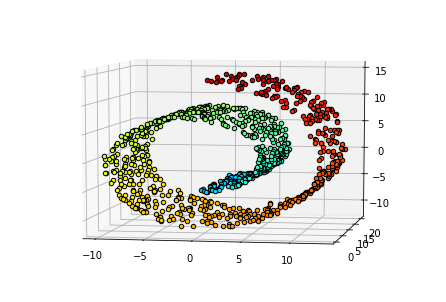
\includegraphics{swissroll.png}}
    \caption{Набор данных Swissroll}
    \label{fig:swissroll}
\end{figure}

Задача визуализации состоит в том, чтобы перевести объекты обратно на двумерную плоскость. Выборка для эксперимента состоит из 1000 точек. Результаты работы методов MDS, Isomap, LLE, t-SNE и UMAP с подобранными\footnote{Здесь и далее: параметры различных методов подбирались так, чтобы достичь адекватного качества визуализации. В некоторых случаях устанавливались дефолтные параметры. Подробнее о влиянии гиперпараметров на качество визуализации смотрите раздел \ref{hparam}.} параметрами изображены на рисунке \ref{fig:resutls_swissroll}.
\begin{figure}[h!]
    \vspace{1em}
    \centering
    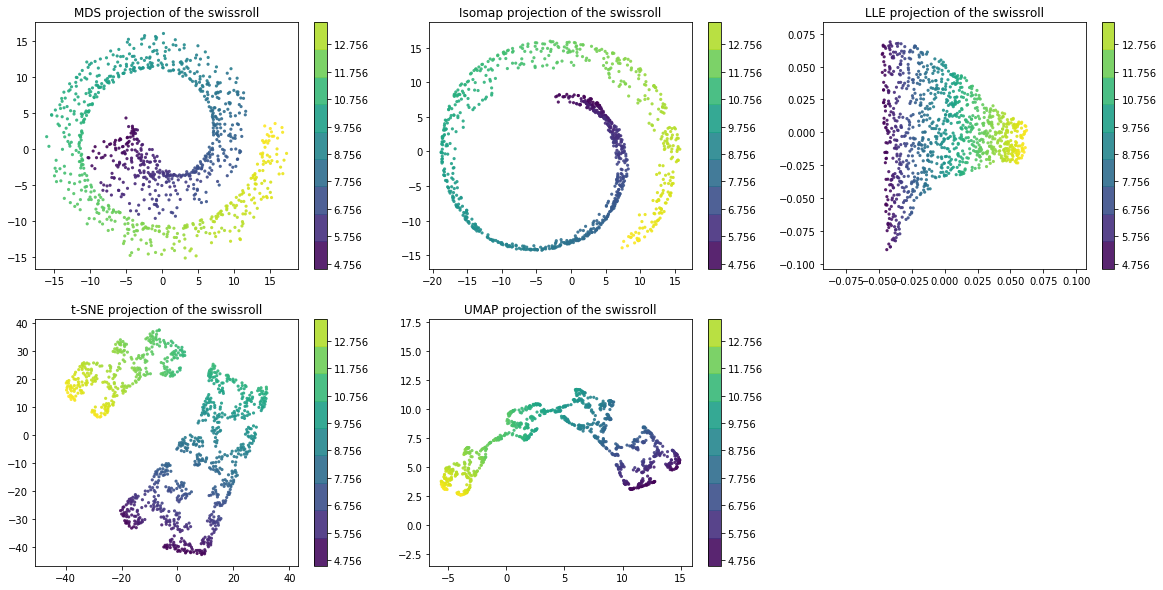
\includegraphics[width=\linewidth]{swissroll_methods.png}
    \caption{Результаты работы методов на наборе данных Swissroll}
    \label{fig:resutls_swissroll}
\end{figure}

Визуально понятно, что более простые методы (MDS и Isomap) при проецировании сохранили геометрическую форму объекта из трёхмерного пространства. Этот результат соответствует принципу их работы: при проецировании на плоскость, параллельную оси $Oz$ на рисунке \ref{fig:swissroll} попарные расстояния между точками остаются наиболее близкими. При этом, границы кластеров чисел разной величины (дискретизированные по colorbar) визуально различимы, и их можно разделить нелинейными кривыми. Проекция LLE практически идеально разделила точки на кластеры в зависимости от их величины, и разделяющие поверхности имеют линейный вид. То же относится и к t-SNE и UMAP, проекции которых, помимо этого, имеют форму полумесяца, то есть эти методы, как и MDS и Isomap, «раскрутили» изначальную спираль данных на двумерной плоскости. Результаты работы TMAP представлены на рисунке \ref{fig:results_swissroll_tmap}. 
\begin{figure}[h!]
    \centering
    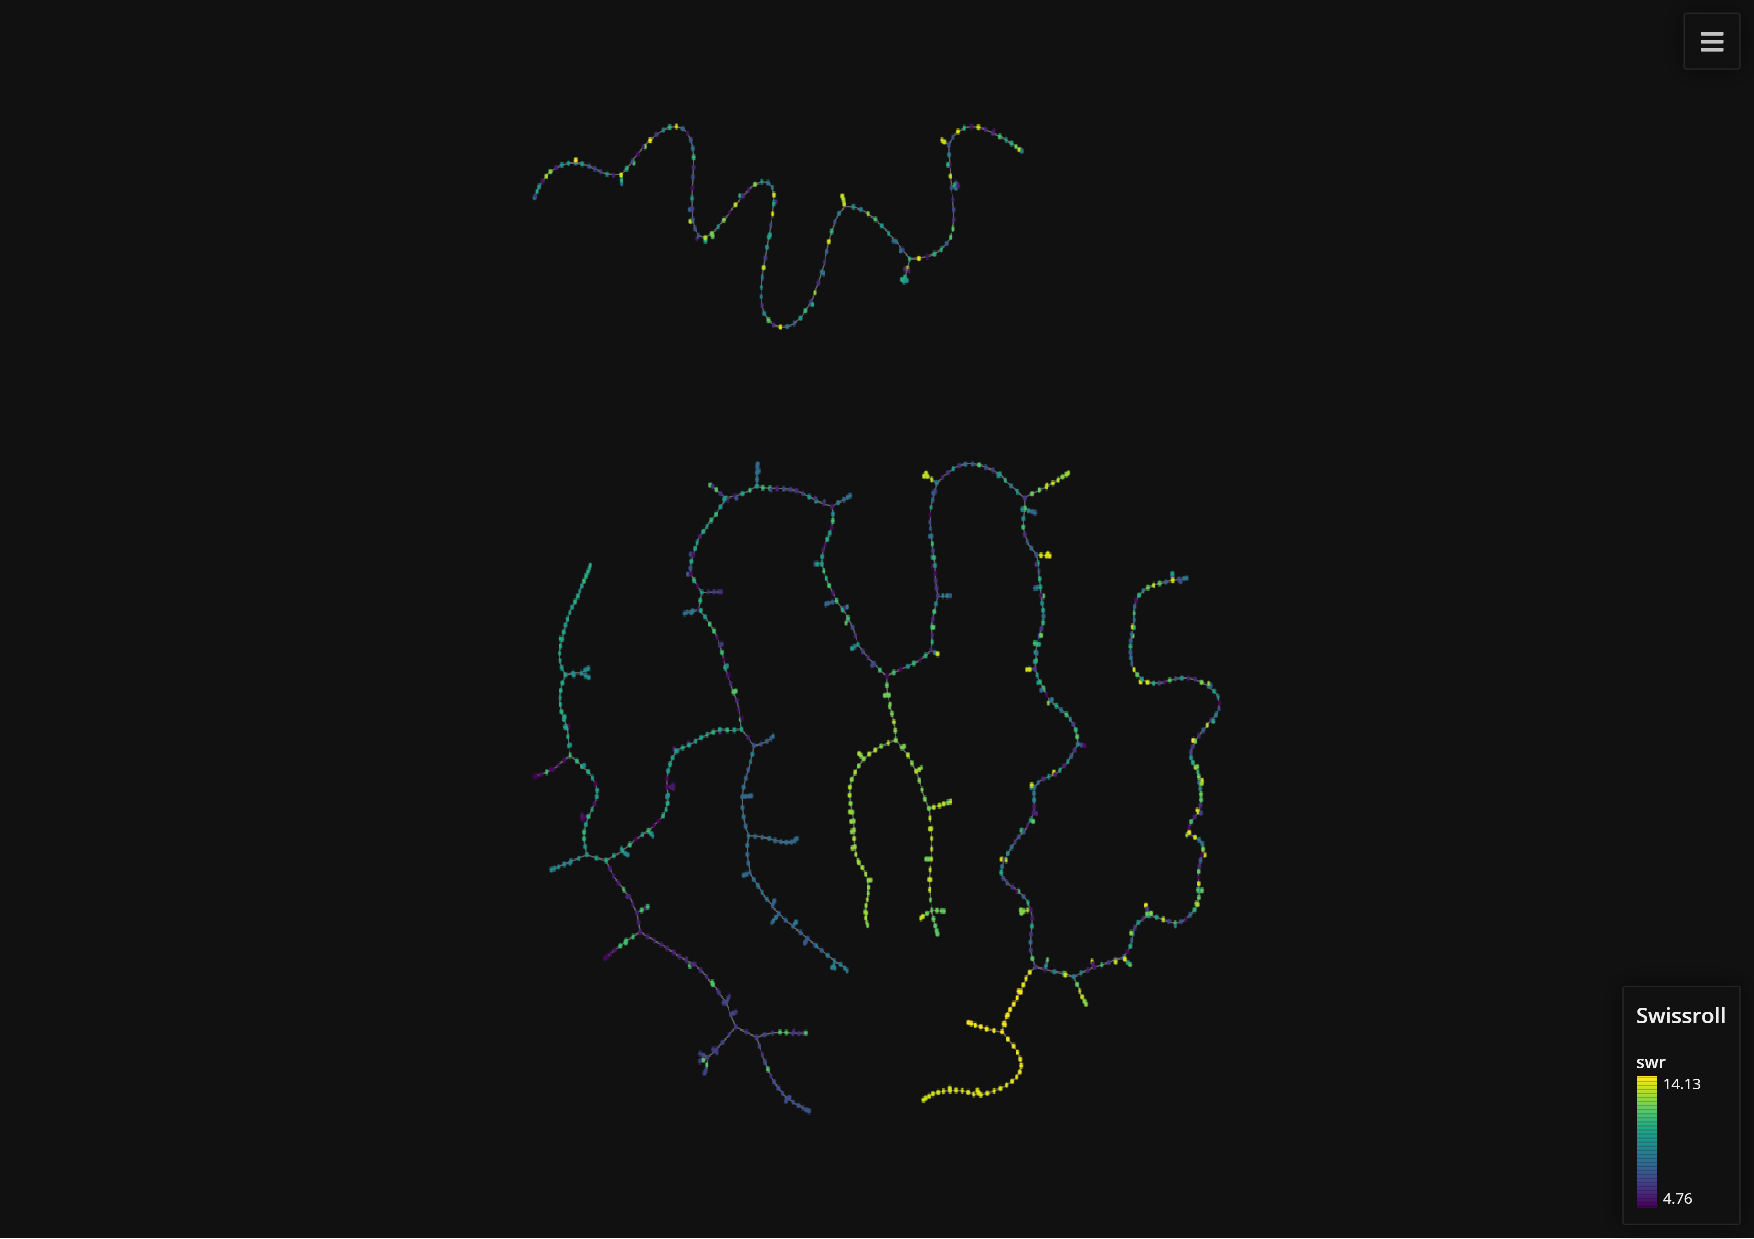
\includegraphics[width=\linewidth]{swissroll_tmap.pdf}
    \caption{Результаты работы TMAP на наборе данных Swissroll}
    \label{fig:results_swissroll_tmap}
\end{figure}

Видно, что в нижней части построенного графа можно выделить кластеры объектов схожей величины, причём близкие по величине кластеры находятся недалеко друг от друга. Например, в левой нижней части графа тёмно-синий кластер переходит в зелёный, как и должно быть. Тем не менее, в правой части графа много неопределённых объектов: жёлтый, синий и зелёный цвета кластеров чередуются в хаотичном порядке. Верхняя компонента графа также состоит из таких неопределённых объектов.

Таким образом, с точки зрения здравого смысла лучший алгоритм зависит от задачи. Если требуется получить двумерную проекцию трёхмерной фигуры так, чтобы эти фигуры были как можно более похожи, то следует выбрать MDS или Isomap. Если же требуется линейно разделить точки, то лучшими варинатами будут LLE, t-SNE и UMAP. TMAP показал худшие результаты\footnote{Хотя и изобразил замечательного кальмара!}, так как не был создан для задач такого типа.

Затраченное время (здесь и далее — на компьютере с AMD A9 Radeon R5, 3.10 GHZ, 8 Gb RAM, Win10 WSL) представлено в таблице \ref{tab:swissroll_time}.

\begin{table}[h!]
    \centering
    \begin{tabular}{l r}
        \toprule
         Алгоритм & Время работы (сек.)  \\
         \midrule
         MDS & 59 \\
         Isomap & 1 \\
         LLE & 0.5 \\
         t-SNE & 8 \\
         UMAP & 15 \\
         TMAP & 2 \\
         \bottomrule
    \end{tabular}
    \caption{Время работы использованных методов на наборе данных Swissroll}
    \label{tab:swissroll_time}
\end{table}

LLE показал лучший результат по времени работы. MDS продемонстрировал худший результат, обрабатывая данные в несколько раз дольше, чем все прочие алгоритмы. 

Описанные выше метрики изображены на рисунке \ref{fig:metrics_swissroll}.
\begin{figure}[h!]
    \centering
    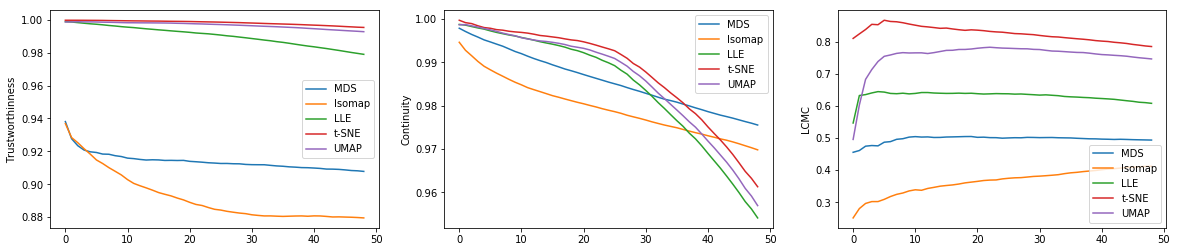
\includegraphics[width=\linewidth]{swissroll_metrics.png}
    \caption{Достоверность, непрерывность и LCMC для методов на наборе данных Swissroll}
    \label{fig:metrics_swissroll}
\end{figure}

При небольшом числе соседей t-SNE занимает лидирующую позицию по всем метрикам, UMAP — второе место, что означает, что эти алгоритмы лучше всего сохранили локальные особенности данных. В глобальном масштабе они также оказались лучшими по достоверности и LCMC, в то время как по непрерывности лучшими стали MDS и Isomap. Такой результат означает, что глобально проекции t-SNE и UMAP не склонны группировать далеко расположенные в исходном пространстве точки (высокая достоверность), но при этом склонны располагать на значительно расстоянии близкие точки (низкая непрерывность). MDS и Isomap стремятся сохранить расстояния в целом, поэтому в глобальном масштабе показывают более хороший результат. 

Таким образом, в совокупности исследованных критериев, лучший алгоритм для проецирования геометрического объекта зависит от задачи. Если требуется сохранить геометрическую форму, следует использовать Isomap. Если требутеся сохранить локальные расстояния между объектами и добиться их линейного разделения по величине, стоит применить LLE, t-SNE или UMAP. В последнем случае, если особо важна скорость работы, LLE является лучшим кандидатом.

\subsection{FASHION MNIST}
 \href{https://www.kaggle.com/zalando-research/fashionmnist}{Набор данных} состоит из чёрно-белых изображений предметов одежды одного из десяти классов. Изображения имеют размер 28$\times$28, то есть общее число признаков равно 784. Задача визуализации — представить набор на двумерной плоскости так, чтобы изображения одного предмета одежды попали в собственный кластер. 
 Набор данных содержит 70 000 картинок.
 Это очень утомительная (или непосильная) задача для большинства приведенных алгоритмов, поэтому в работе 
 для получения визуализаций использовалась случайная подвыборка из 3 500 наблюдений.
 Стоит отметить, что на обработку полного набора данных у UMAP уходит около 5 минут, то есть этот алгоритм, в отличие от многих, пригоден для эффективной работы с большими наборами данных.
 
 Результаты работы методов MDS, Isomap, LLE, t-SNE и UMAP с дефолтными параметрами изображены на рисунке \ref{fig:resutls_fmnist}.
 \begin{figure}[h!]
    \vspace{1em}
    \centering
    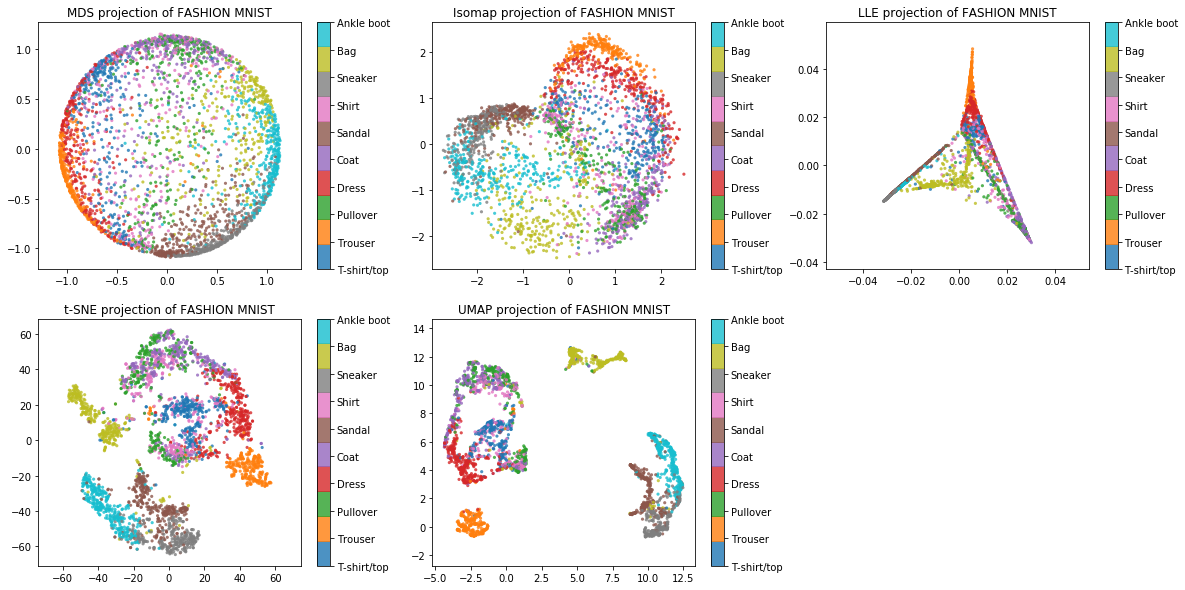
\includegraphics[width=\linewidth]{fmnist_methods.png}
    \caption{Результаты работы методов на наборе данных FASHION MNIST}
    \label{fig:resutls_fmnist}
\end{figure}

Видно, что MDS, Isomap и LLE достаточно плохо справились с задачей\footnote{Тем не менее, мыльный пузырь и сердце получились восхитительными!}: на проекциях визуально различимы некоторые кластеры (брюки и платья), однако границы сильно размыты, и разделяющая поверхность имеет сложный нелинейный вид. Есть и кластеры (сумки для MDS, рубашки для Isomap, ботильоны для LLE), оказавшиеся неотделимыми. t-SNE показал более хороший результат: с небольшой ошибкой можно отделить ботильоны, сандалии, сникеры, брюки, футболки, сумки и платья. Свитеры и плащи оказались неразделимыми, что является логически приемлемым. UMAP также хорошо отделил сумки, ботильоны, брюки, платья и футболки, но свитеры и плащи, а также сникеры и сандалии оказались неразделимыми. Результаты работы TMAP представлены на рисунке \ref{fig:tmap_fmnist}. 
 \begin{figure}[h!]
    \vspace{1em}
    \centering
    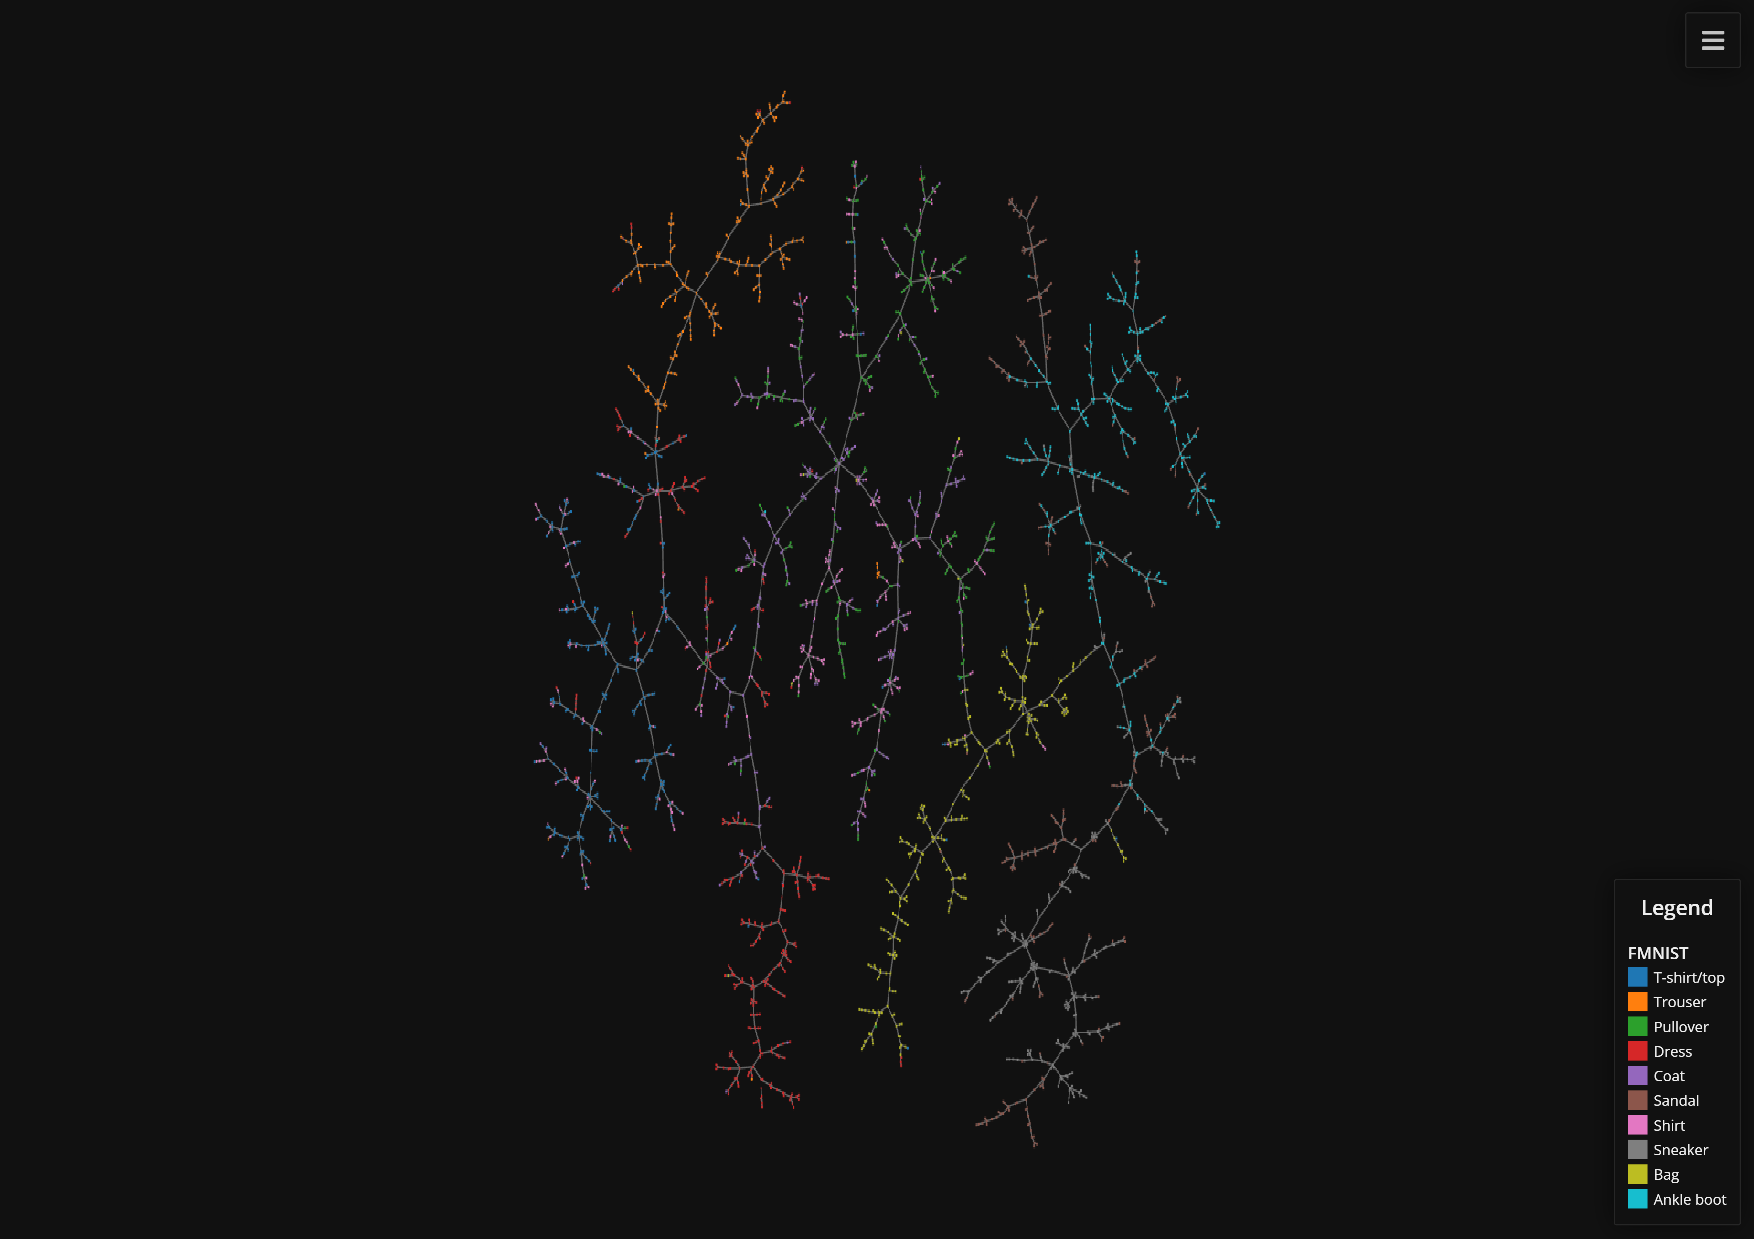
\includegraphics[width=\linewidth]{fmnist_tmap.pdf}
    \caption{Результаты работы TMAP на наборе данных FASHION MNIST}
    \label{fig:tmap_fmnist}
\end{figure}

Полученный граф достаточно хорошо решает задачу: отчётливо разделимы брюки, ботильоны и сумки. Как и в случае UMAP, сандалии и сникеры и свитеры и плащи оказались смешаны. В целом, граф достаточно похож на проекцию UMAP в плане расположения кластеров, например, платья и футболки лежат близко к плащам и свитерам, а последние находятся далеко от брюк. 

Затраченное время представлено в таблице \ref{tab:fmnist_time}.
\begin{table}[h!]
    \centering
    \begin{tabular}{l r}
        \toprule
         Алгоритм & Время работы (сек.)  \\
         \midrule
         MDS & 1002 \\
         Isomap & 43 \\
         LLE & 22 \\
         t-SNE & 52 \\
         UMAP & 25 \\
         TMAP & 25 \\
         \bottomrule
    \end{tabular}
    \caption{Время работы использованных методов на наборе данных FASHION MNIST}
    \label{tab:fmnist_time}
\end{table}

LLE показал лучший результат по времени. Примечательно, что t-SNE, проекция которого лучше всего разделяет классы, компенсирует качество визулизации временем работы, более чем в два раза превышающем прочие методы, кроме MDS. Последний выделяется: если все прочие алгоритмы работают в пределах минуты, то MDS выполняется за 15-20 минут. 

Метрики изображены на рисунке \ref{fig:metrics_fmnist}.
\begin{figure}[h!]
    \centering
    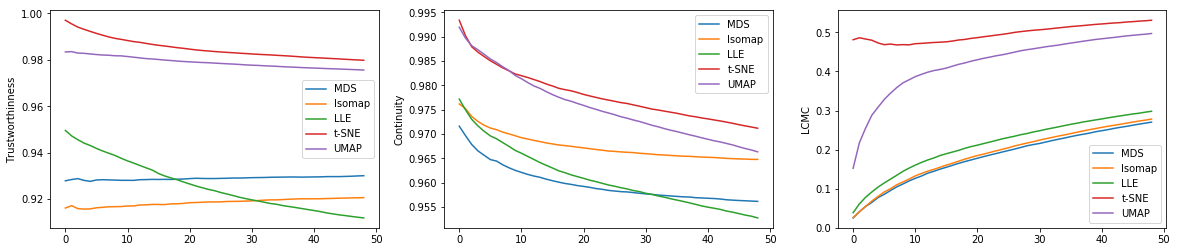
\includegraphics[width=\linewidth]{fmnist_metrics.png}
    \caption{Достоверность, непрерывность и LCMC для методов на наборе данных FASHION MNIST}
    \label{fig:metrics_fmnist}
\end{figure}

В данном случае по всем метрикам и локальные, и глобальные связи лучше всего сохраняет t-SNE, на втором месте — UMAP. 

Таким образом, в задаче визуализации изображений для последующей кластеризации лучшее качество показал t-SNE как на основе здравого смысла, так и по метрикам. Тем не менее, время его работы оказалось в два раза больше, чем у UMAP, который справился с задачей лишь немного хуже. Поэтому если в выборе между временем работы и точностью важно первое, следует использовать UMAP, если второе, то t-SNE. Отдельно стоит упомянуть, что TMAP также показал хорошие результаты и сопоставим с UMAP как по качеству визуализации, так и по времени работы.

\subsection{News Aggregator Dataset}

\href{https://www.kaggle.com/uciml/news-aggregator-dataset}{Набор данных} содержит заголовки новостей, собранные сетевым аггрегатором с марта по август 2014 года. 
Каждый заголовок является предложением, которое относится к одной из четырёх категорий: бизнес, науки и технологии, развлечения и здоровье. Задача визуализации состоит в том, чтобы представить эти предложения на двумерной плоскости так, чтобы рядом оказались заголовки из одной категории.

Перед применением алгоритмов визуализации, предложения были лемматизированы, очищены от стоп-слов и векторизированы при помощи TF-IDF. Стоит отметить, что в оригинальном наборе данных содержится более 422 тыс. предложений, но для эксперимента была взята случайная подвыборка из 1000 наблюдений, так как обработка даже 5 тыс. объектов оказалась очень времязатратной для MDS и t-SNE.
Результаты работы методов MDS, Isomap, LLE, t-SNE и UMAP с дефолтными параметрами изображены на рисунке \ref{fig:resutls_news}.
\begin{figure}[h!]
    \vspace{1em}
    \centering
    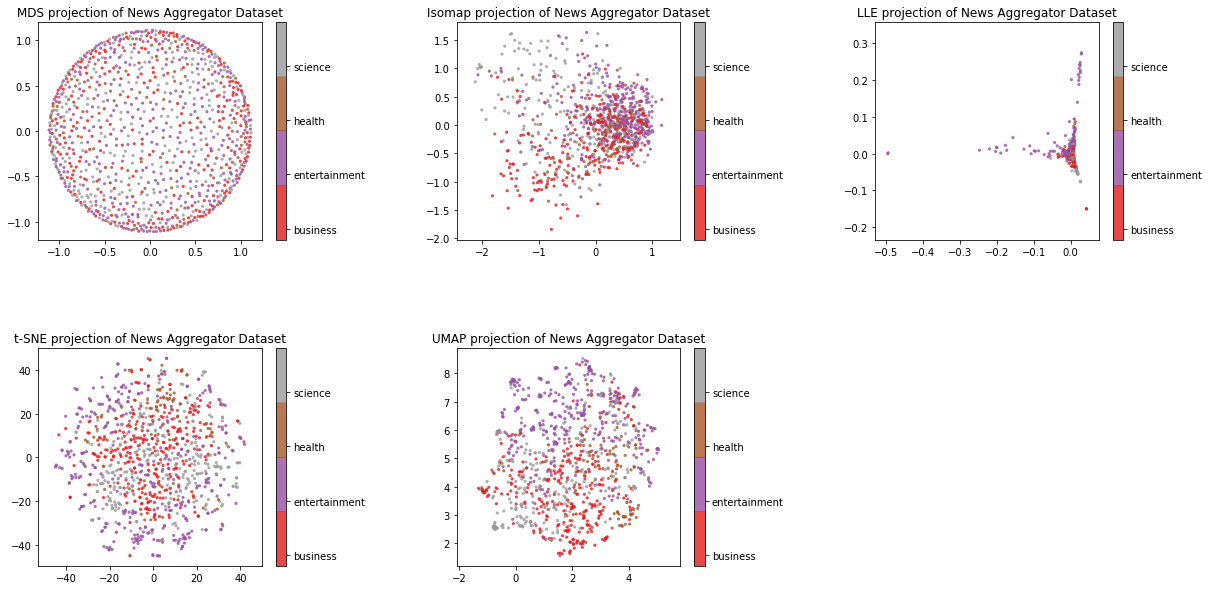
\includegraphics[width=\linewidth]{news_methods.png}
    \caption{Результаты работы методов на наборе данных News Aggregator Dataset}
    \label{fig:resutls_news}
\end{figure}

Все алгоритмы отработали плохо: ни один не позволяет разделить предложения по категориям. TMAP, показал сходие результаты, которые представлены на рисунке \ref{fig:tmap_news}. Видно, что алгоритм также не справился с задачей: примерно отделимы только предложения, относящиеся к категории здоровья. Все прочие категории оказались неразделимы. 
\begin{figure}[h!]
    \vspace{1em}
    \centering
    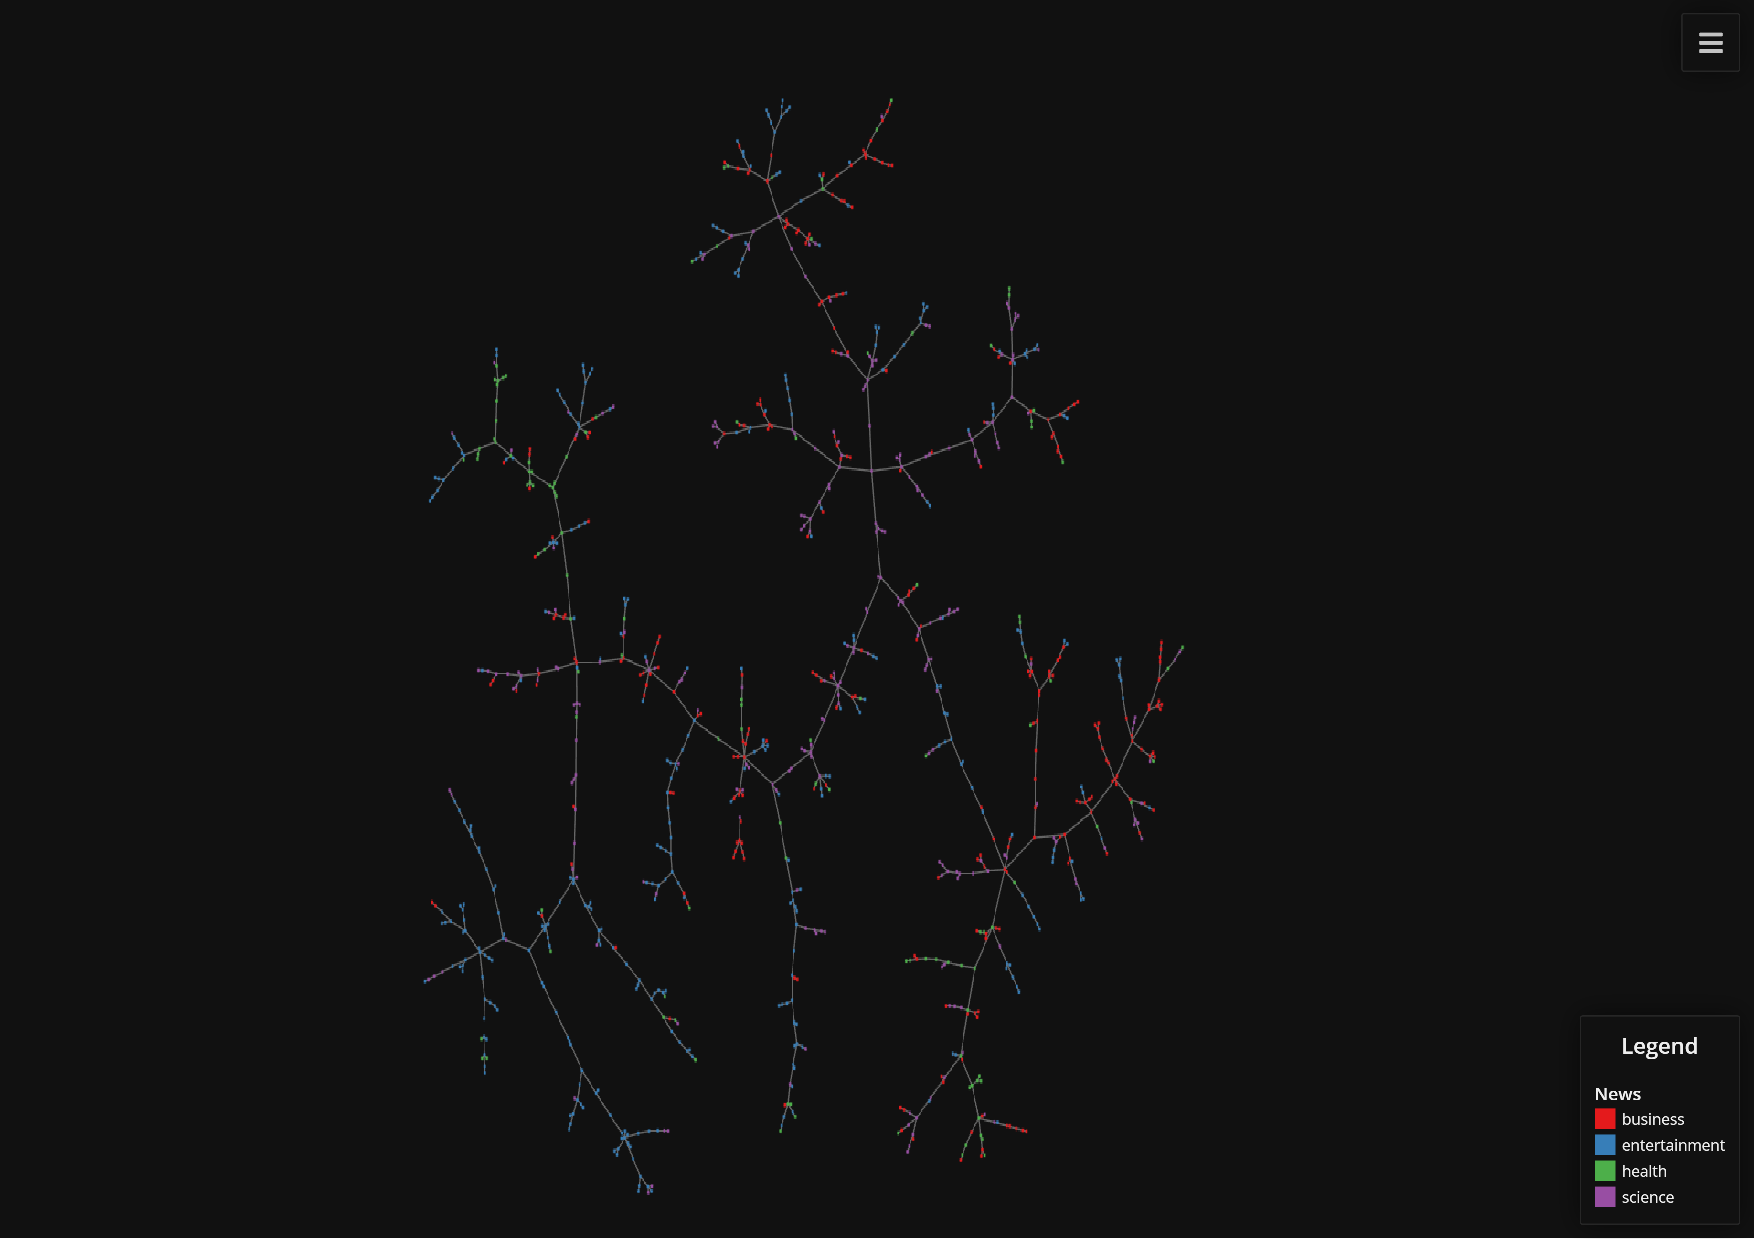
\includegraphics[width=\linewidth]{news_tmap.pdf}
    \caption{Результаты работы TMAP на наборе данных News Aggregator}
    \label{fig:tmap_news}
\end{figure}
Затраченное время представлено в таблице \ref{tab:news_time}.
\begin{table}[h!]
    \centering
    \begin{tabular}{l r}
        \toprule
         Алгоритм & Время работы (сек.)  \\
         \midrule
         MDS & 22 \\
         Isomap & 13 \\
         LLE & 13 \\
         t-SNE & 22 \\
         UMAP & 6 \\
         TMAP & 31 \\
         \bottomrule
    \end{tabular}
    \caption{Время работы использованных методов на наборе данных News Aggregator Dataset}
    \label{tab:news_time}
\end{table}
Лучшим по времени оказался UMAP. Примечательно, что в отличие от других наборов, время работы MDS сопоставимо с другими алгоритмами.

Метрики изображены на рисунке \ref{fig:metrics_news}.
\begin{figure}[h!]
    \centering
    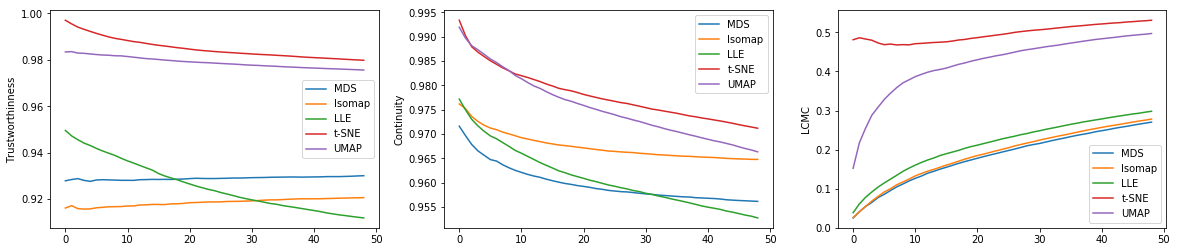
\includegraphics[width=\linewidth]{fmnist_metrics.png}
    \caption{Достоверность, непрерывность и LCMC для методов на наборе данных News Aggregator Dataset}
    \label{fig:metrics_news}
\end{figure}
На основании метрик лучшее качество показали t-SNE и UMAP как в локальном, так и в глобальном масштабах. Тем не менее, в данном случае разумным кажется полагаться на здравый смысл, а не на метрики: все алгоримы не справились с поставленной задачей. 

Таким образом, ни один алгоритм не справился с визуализацией на текстах. Чтобы устранить эффект влияния качества набора данных, эксперимент был повторён на стандартном корпусе текстов из \code{sklearn} \href{http://qwone.com/~jason/20Newsgroups/}{20 Newsgroups}. Набор содержит 20 000 постов из 20 новостных групп, соответствующих разным темам. 
На этом наборе были протестированы методы, показавшие себя лучшими в предыдущих задачах: t-SNE и UMAP. Результаты приведены на рисунке \ref{fig:firework}.

\begin{figure}[h!]
    \vspace{1em}
    \centering
    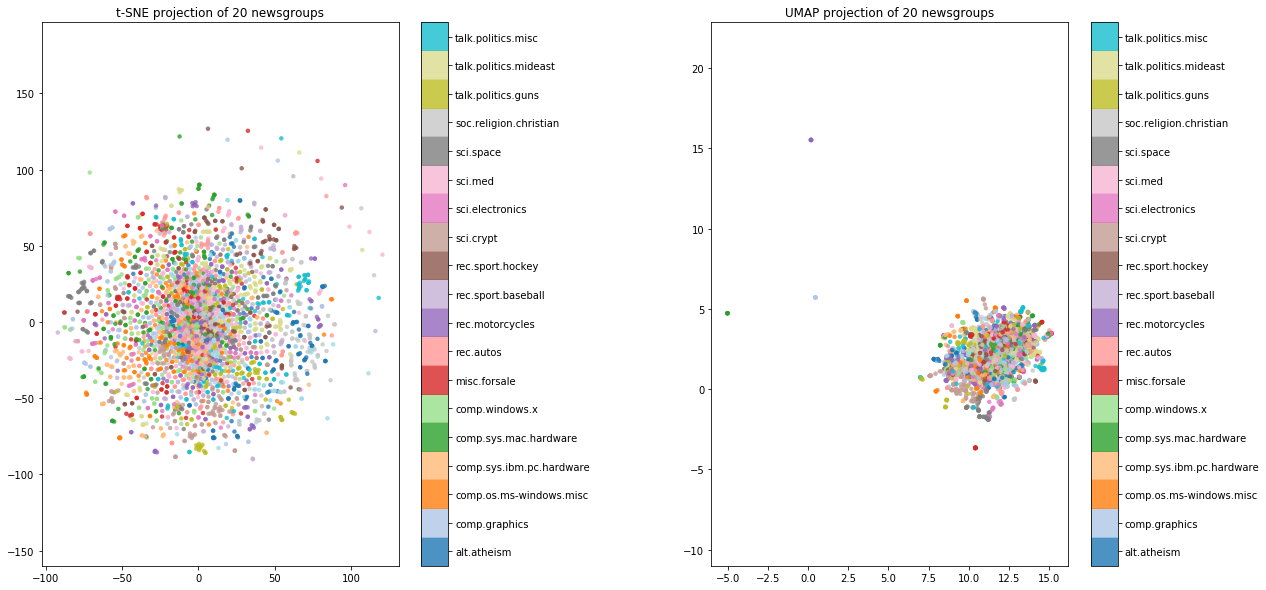
\includegraphics[width=\linewidth]{fireworks.png}
    \caption{Результаты работы t-SNE и UMAP на наборе данных 20 Newsgroup}
    \label{fig:firework}
\end{figure}

К сожалению, эксперимент провалился: алгоритму не удалось выделить классы новостей по тематикам. Можно сделать вывод о том, что рассмотренные методы визуализации плохо работают на текстовых данных, во всяком случае при использовании выборок небольших размеров.

\section{Настройка гиперпараметров}\label{hparam}

В этом разделе проиллюстрировано, как меняется качество визуализации описанных алгоритмов в зависимости от значений гиперпараметров. Все эксперименты были проведены на наборе данных FASHION MNIST. Влияние гиперпараметров на качество визуализации MDS не рассматривалось, так как стоит признать, что этот алгоритм является бесспорным аутсайдером\footnote{\, :)}. При этом время его работы даже на небольшой выборке велико. Для экономии места изображения для тестирования TMAP вынесены в код. Для этого алгоритма изменялись размер векторов MinHash и число префиксных деревьев в LSH Forest. Было получено, что в целом, качество визуализации остаётся примерно одинаковым: меняется струкутра деревьев и расположение в них классов, однако чёткость их выделения и логика расположения сохраняются.

Для всех остальных методов рассмотривается параметр \code{n\_neighbors} (для t-SNE — \code{perplexity}), регулирующий число соседей в окрестности многообразия для каждой точки.
Как правило, этот параметр оказывает наибольшее влияние на визуализацию, так как устанавливает баланс между сохранением локальных и глобальных особенностей исходного признакового пространства.

На рисунках \ref{fig:isomap_mnist} — \ref{fig:umap_mnist} представлены визуализации работы алгоритмов при разных значениях гиперпараметров.

\begin{figure}[htp!]
    \centering
    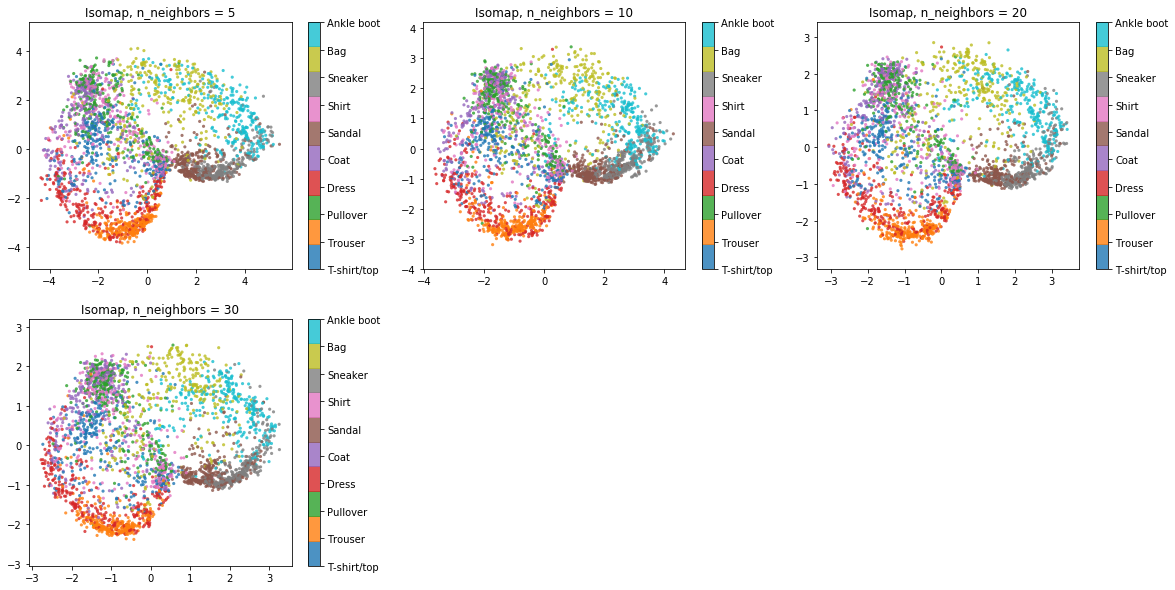
\includegraphics[width=\linewidth]{isomap_mnist.png}
    \caption{Isomap-визуализация FMNIST}
    \label{fig:isomap_mnist}
\end{figure}

\begin{figure}[htp!]
    \centering
    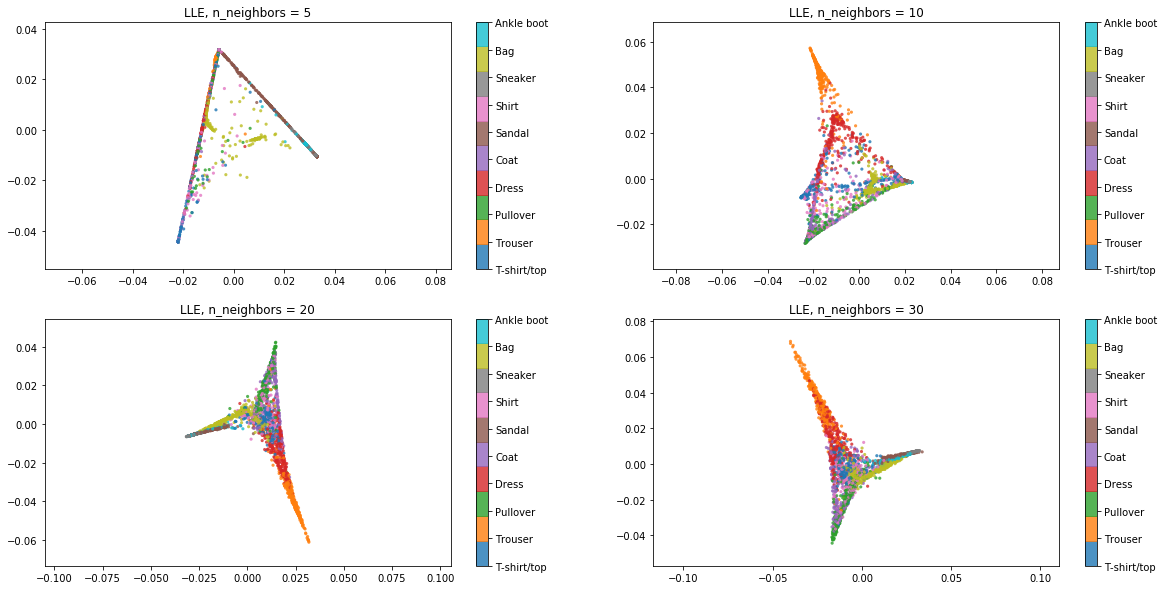
\includegraphics[width=\linewidth]{lle_mnist.png}
    \caption{LLE-визуализация FMNIST}
    \label{fig:lle_mnist}
\end{figure}

Визуализация с помощью Isomap (рисунок \ref{fig:isomap_mnist}) практичеcки не меняется при различных значениях параметра.
Изменения можно заметить, только наблюдая за отдельными точками.
Художественные возможности алгоритма поражают, однако границы классов остаются размытыми, а некоторые отдельные классы сильно перемешаны, например, платья (красные точки) и брюки (оранжевые точки).

В случае LLE (рисунок \ref{fig:lle_mnist}) качество визуализации явно растет при больших значениях гиперпараметра.
Данные хорошо группируются по кластерам, однако все кластеры находятся близко друг к другу.

\begin{figure}[t!]
    \vspace{1em}
    \centering
    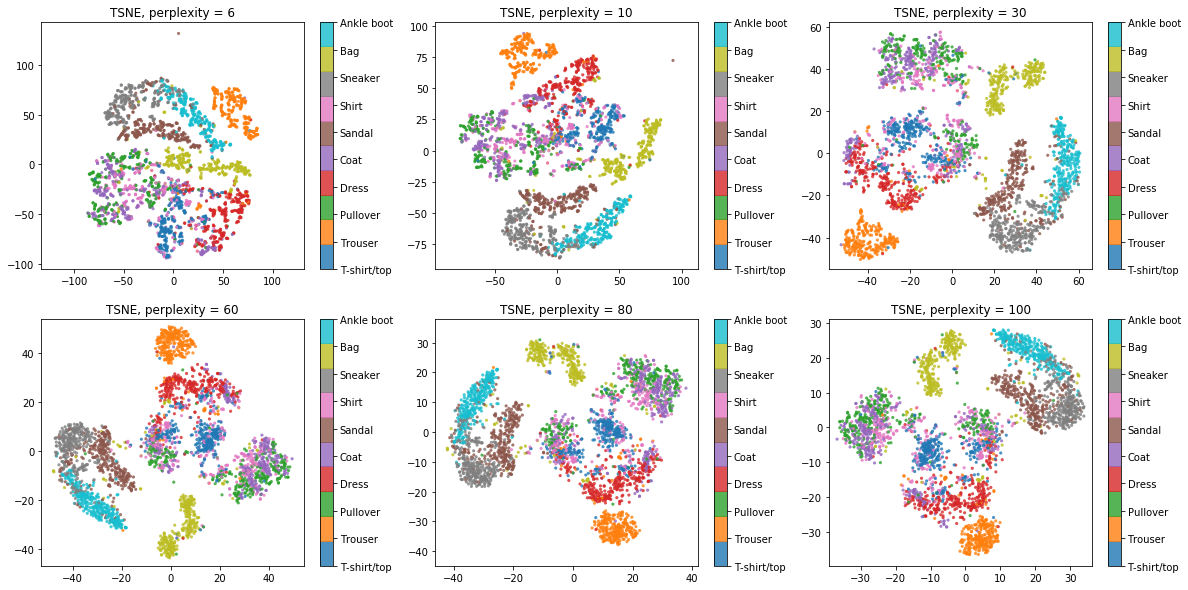
\includegraphics[width=\linewidth]{tsne_mnist.png}
    \caption{t-SNE-визуализация FMNIST}
    \label{fig:tsne_mnist}
\end{figure}

Как правило, для t-SNE классическая рекомендация — использовать б\'ольшие значения параметра \\ \code{perplexity} для больших наборов данных.
На примере подвыборки из FMNIST (рисунок \ref{fig:tsne_mnist}) видно, что при маленьких значениях параметра «облака» классов оформлены плохо.
С ростом значения \code{perplexity} классы отдельных видов одежды располагаются друг от друга дальше, то есть алгоритм лучше учитывает глобальную структуру данных.
Значение параметра около 60 кажется оптимальным.

\begin{figure}[h!]
    \vspace{1em}
    \centering
    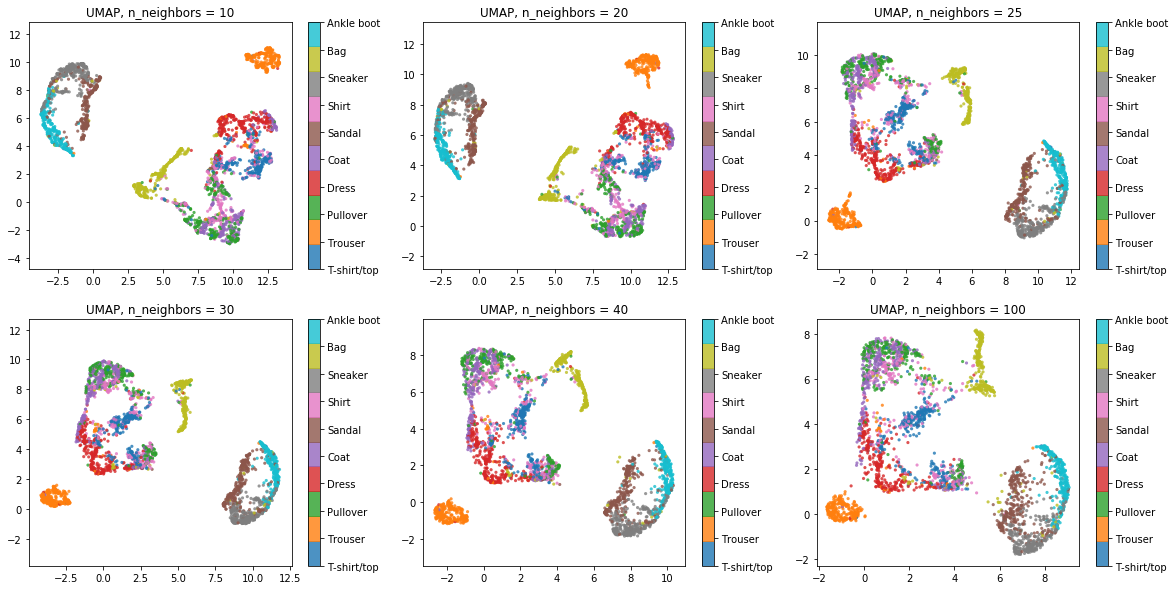
\includegraphics[width=\linewidth]{umap_mnist.png}
    \caption{UMAP-визуализация FMNIST}
    \label{fig:umap_mnist}
\end{figure}


В случае UMAP (рисунок \ref{fig:umap_mnist}) визуально кажется, что значимых улучшений при различных значениях параметра нет.
Тем не менее, слишком большое число соседей приводит к тому, что границы классов становятся размытыми.

\begin{shaded}
Таким образом, результаты экспериментов показывают, что лучшими при решении различных задач оказались t-SNE и UMAP. Первый выигрывает в качестве визуализации, а второй — в её скорости, при этом не сильно уступая t-SNE по качеству. Линейный MDS оказался хуже всех прочих методов по обоим показателям. TMAP, сопоставимый по времени работы с UMAP, проигрывает на некоторых стандартных наборах данных по качеству визуализации, так как  был создан в первую очередь для решения специфических научных задач.
\end{shaded}

\newpage

\printbibliography

\end{document}